A major challenge in reconfigurable atomic services is to examine the latency of terminating read and write operations, especially when those are invoked concurrently with reconfiguration operations. 
In this section we provide an in depth analysis of the latency of operations in \ares{}. Additionally, a storage and communication analysis is shown when \ares{} utilizes 
the erasure-coding algorithm presented in Section \ref{ssec:dap:impl}, in each configuration. 

% of the storage and communication costs of \ares{}, 
% and the latency of read and write operations. 

\subsection{Latency Analysis}
\label{sec:safety:d}
Liveness (termination) properties cannot be specified for ~\ares{}, without restricting asynchrony  or the
rate of arrival of \act{reconfig} operations, or if the consensus protocol never terminates.
Here,  we provide some conditional performance analysis of the operation, based on 
%assumptions on the 
latency bounds on the message \nnrev{delay}{delivery}. %in the network.
 We assume that local computations take negligible time and the latency of an 
operation is  due to the delays in the messages exchanged during the execution. 
%Before proceeding with our 
%analysis we define an upper and lower communication bounds. 
We measure delays in \myemph{time units} of some global clock, which is visible only to an external viewer.
No process has access to the clock.
Let $\smdelay$ and $\lgdelay$ be the minimum and maximum durations taken by 
 messages, sent during an execution  of~\ares,  to reach their destinations.
%denote the minimum message delivery delay 
%between any two processes in the service; let $\lgdelay$ be the 
%maximum delivery delay. 
 Also, let $\opdelay{\op}$ denote the duration 
 of an operation (or action) $\op$. In the statements that follow, 
 we consider any execution $\EX$ of \ares, which contains $k$ \act{reconfig} operations.
 \kmk{For any configuration $c$ in an execution of~\ares{},  we assume that any 
 	$\consensus{c}.\act{propose}$ operation, takes at least $\opdelaymin{CN}$ time units.}


\remove{
\begin{lemma}
\label{lem:opdelays}
Suppose $\pi$ and $\phi$ are operations of the type \act{put-config}, \act{read-next-config}, respectively, invoked by some non-faulty reconfiguration clients,  then the latency of these operations are bounded as follows: 
%\begin{itemize}
	%\item 
	$(i)$ $2\smdelay\leq \opdelay{\pi}\leq 2\lgdelay$
	%\item 
	and 
	$(ii)$ $2\smdelay\leq \opdelay{\phi}\leq 2\lgdelay$.
%\end{itemize}
\end{lemma}
}
Let us first examine what is the action delays based on the boundaries we assume. 
It is easy to see that actions \act{put-config}, \act{read-next-config} perform two message exchanges thus take time $2\smdelay\leq \opdelay{\phi}\leq 2\lgdelay$. 
From this we can derive the delay of  a \act{read-config} action.

\begin{lemma}
	\label{lem:rcdelay}
	Let $\phi$ be a $\act{read-config}$ operation invoked by a non-faulty reconfiguration client $\rec$, 
	with the input argument and returned values of $\phi$ as  $\cvec{\rec}{\st}$ and  $\cvec{\rec}{\st'}$ respectively. Then the delay of $\phi$ is:	$4\smdelay(\nu(\cvec{\rec}{\st'})-\mu(\cvec{\rec}{\st})+1)\leq \opdelay{\phi}\leq4\lgdelay(\nu(\cvec{\rec}{\st'})-\mu(\cvec{\rec}{\st})+1)$.
    %$4\smdelay(\nu-\mu+1)\leq \opdelay{\phi}\leq 4\lgdelay(\nu-\mu+1)$.
\end{lemma}

From Lemma \ref{lem:rcdelay} it is clear that the latency of a $\act{read-config}$ action 
depends on the number of configurations installed since the last  finalized configuration known to the recon client.

% \remove{
% Let $\seqlen = \nu-\mu$ denote the number of newly installed configurations.
% %Now let us examine when a new configuration gets inserted in the configuration 
% %sequence by a \act{reconfig} operation.
Given the latency of a \act{read-config}, we can compute the minimum amount 
of time it takes for $k$ configurations to be installed.

% \begin{lemma}
% 	\label{lem:configdelay}
% 	Let $\sigma$ be the last state of a fair execution of \ares{}, $\EX$. 
% 	Then $k$ configurations can be installed to $\cvec{}{\sigma}$, in time no less than
% %	\begin{equation}
% 	$ \left(\opdelaymin{CN}+6\smdelay\right)k$.
% %	\end{equation}
% 	%by the completion of its $\act{add-config}$ action 
% %	in our execution construction.
% \end{lemma}
% \begin{proof}
% 	Figure \ref{fig:reconfigExec} shows the timings of each reconfiguration operation. 
% 	In particular, consider the first reconfiguration $\rec_1$. During its $\act{read-config}$
% 	$\rec_1$ does not discover new configurations and thus, if $seq_1$ is the input and 
% 	$seq'_1$ the output configuration, $\mu(seq_1)=\nu(seq'_1)$. Thus, by Lemma \ref{lem:rcdelay},
% 	the $\act{read-config}$ takes at least time $4\smdelay$. Since the consensus algorithm 
% 	takes $\opdelay{CN}$ and the $\act{put-config}$ action at least $2\smdelay$,
% 	then $\rec_1$ takes time at least $\opdelay{\rec_1} \geq 4\smdelay + \opdelaymin{CN} + 2\smdelay$
% 	to install configuration $c_1$. So without counting the time that each subsequent reconfigurer 
% 	takes to discover the newly introduced configurations, for $k$ configurations to be installed
% 	in the sequence will take no less than $k(6\smdelay + \opdelaymin{CN})$ completing our proof.
% \end{proof}

\remove{
 In \ares{} a \act{reconfig} operation has 
four phases: $(i)$ $\act{read-config}(cseq)$,  reads the latest configuration sequence, 
$(ii)$ $\text{\act{add-config}}(cseq, c)$,  attempts to add  the new configuration 
at the end of the global sequence $\mathcal{G}_L$, 
$(iii)$ $\text{\act{update-config}}(cseq)$,   transfers the knowledge to the added configuration,
and 
$(iv)$  $\text{\act{finalize-config}}(cseq)$ finalizes the added configuration. 

%So, a new configuration is appended to the 
%end of the configuration sequence (and it becomes visible to any operation) during the 
%\act{add-config} action. 
 During the execution of \act{add-config} action, the recon client proposes to a consensus 
service  
to learn the configuration to accept, and then invokes a \act{put-config} action notify a quorum of servers in the configuration of the  decided configuration. 
%Any operation that is invoked after the \act{put-config} action 
%will observed the newly added configuration. 

When multiple reconfiguration operations  are invoked concurrently, each at a separate client, then it is possible 
that each of the clients  successfully append their  new  configurations to the end of $\mathcal{G}_L$. 
This is possible when 
the \act{read-config} action of each \act{reconfig} operation begins  after the completion of  \act{put-config}
action of another \act{reconfig} operation. 
}

%Next we 
The following lemma shows the maximum latency of a read or a write operation, invoked by any non-faulty client. 
From~\ares{} algorithm,  the latency of a read/write operation depends on the delays of the  DAPs  operations. 
%influence  the delay of a read and write operation. 
For our analysis we assume 
that all $\act{get-data}$, $\act{get-tag}$ and $\act{put-data}$ primitives use 
two phases of communication.  Each phase consists of a communication between the client and the servers.
%\kmkremove{Such an assumption is justified by atomic algorithms like ~\treas{} and ABD. }

\begin{lemma}
	\label{lem:dapdelays}
Suppose $\pi$,  $\phi$ and $\psi$ are operations of the type \act{put-data}, \act{get-tag} and  \act{get-data}, respectively, invoked by some non-faulty reconfiguration clients,  then the latency of these operations are bounded as follows: 
	$(i)$ $2\smdelay\leq \opdelay{\pi}\leq 2\lgdelay$; $(ii)$
	 $2\smdelay\leq \opdelay{\phi}\leq 2\lgdelay$; and $(iii)$
	  $2\smdelay\leq \opdelay{\psi}\leq 2\lgdelay$.
\end{lemma}
%Now we show the delay of a read or a write operation $\op$.

In the following lemma, we estimate the time taken for a read or a write operation to complete,
	when it discovers $k$ configurations between its invocation and response steps.
%
%show that in a fair execution of ~\ares{} \nnrev{where there are at}{that contains} $k$ reconfiguration 
%operations, any read or write operation takes at most  $6\lgdelay\left(k+2\right)$.
 

\begin{lemma}
	\label{lem:rwdelay}
%Consider a execution of ~\ares{} where there are $k$ reconfiguration and a read or a write operation $\pi$ invoked by a non-faulty then   $6\lgdelay(k+1)$.
Consider any  execution of ~\ares{} where at most  $k$ reconfiguration operations are invoked.
Let $\sigma_s$ and $\sigma_e$ be the states before the invocation 
and after the completion step of a read/write operation $\op$,
in some fair execution $\EX$ of \ares{}. 
%If $k=\nu(\cvec{\pr}{\sigma_e}) - \mu(\cvec{\pr}{\sigma_s})$, 
Then we have 
$\opdelay{\op}\leq 6\lgdelay\left(k+2\right)$ to complete. 
\end{lemma}

\begin{proof}
	Let $\state_s$ and $\state_e$ be the states before the invocation 
	and after the completion step of a read/write operation $\op$ by $\pr$ respectively,
	in some execution $\EX$ of \ares. 
	%Then $\op$ takes time at most:
%	\[
%		\opdelay{\op}\leq 6\lgdelay\left[\nu(\cvec{\pr}{\state_e}) - \mu(\cvec{\pr}{\state_s})+2\right]
%	\] 
	By algorithm examination we can 
	see that any read/write operation performs the following actions in this order:
	$(i)$  \act{read-config}, $(ii)$ \act{get-data} (or \act{get-tag}), $(iii)$ \act{put-data},
	and $(iv)$ \act{read-config}. Let $\state_1$ be the state when the first \act{read-config}, denoted by $\act{read-config}_1$, 
	action terminates. By Lemma \ref{lem:rcdelay} the action will take time:
	\[
		\opdelay{\act{read-config}_1} \leq 4\lgdelay(\nu(\cvec{\pr}{\state_1})-\mu(\cvec{\pr}{\state_s})+1)
	\]
	The $\act{get-data}$ action that follows the \act{read-config} (Lines Alg.~\ref{algo:writer}:\ref{line:rw:getdata:start}-\ref{line:rw:getdata:end}) also took at most $(\nu(\cvec{\pr}{\state_1})-\mu(\cvec{\pr}{\state_s})+1)$ time units,
	given that no new finalized configuration was discovered by the \act{read-config} action. 
	Finally, the \act{put-data}  and the second \act{read-config} actions of $\op$ may be invoked at most
	$(\nu(\cvec{\pr}{\state_e})-\nu(\cvec{\pr}{\state_1})+1)$ times, given that the \act{read-config} action discovers 
	one new configuration every time it runs. Merging all the outcomes, the total time of $\op$ can be at most:
	\begin{eqnarray*}
	\opdelay{\op} & \leq & 4\lgdelay(\nu(\cvec{\pr}{\state_1})-\mu(\cvec{\pr}{\state_s})+1) + 2\lgdelay(\nu(\cvec{\pr}{\state_1})-\mu(\cvec{\pr}{\state_s})+1) + (4\lgdelay+2\lgdelay)(\nu(\cvec{\pr}{\state_e})-\nu(\cvec{\pr}{\state_1})+1) \\
%	 & \leq & 6\lgdelay\nu(\cvec{\pr}{\state_1})-6\lgdelay\mu(\cvec{\pr}{\state_s})+6\lgdelay\nu(\cvec{\pr}{\state_e})-6\lgdelay\nu(\cvec{\pr}{\state_1})+12\lgdelay \\
	 & \leq & 6\lgdelay\left[\nu(\cvec{\pr}{\state_e}) - \mu(\cvec{\pr}{\state_s})+2\right] \leq 6D(k+1)
	\end{eqnarray*}
where  $\nu(\cvec{\pr}{\state_e}) - \mu(\cvec{\pr}{\state_s})\leq k + 1$ since there can be at most $k$ new configurations installed. and the result of the lemma follows.
\end{proof}

It remains now to examine the conditions under which a read/write operation may “catch up” with an infinite number of reconfiguration operations.
For the sake of a worst case analysis we will assume that reconfiguration operations suffer 
the minimum delay $d$, whereas read and write operations suffer the maximum
delay $D$ in each message exchange. 
% Also, we assume that any consensus operation takes the least amount of time to complete $\opdelaymin{CN}$.
We first show how long it takes for $k$ configurations to be installed.

\begin{lemma}
	\label{lem:configdelay}
	Let $\sigma$ be the last state of a fair execution of \ares{}, $\EX$. 
	Then $k$ configurations can be installed to $\cvec{}{\sigma}$, in time
	$\opdelay{k} \geq 4\smdelay\sum_{i=1}^{k}i+ k\left(\opdelaymin{CN}+2\smdelay\right)$ time units.
%	\begin{equation}
	%$ \left(\opdelaymin{CN}+6\smdelay\right)k$.
%	\end{equation}
	%by the completion of its $\act{add-config}$ action 
%	in our execution construction.
\end{lemma}

\begin{proof}
    In \ares{} a \act{reconfig} operation has 
four phases: $(i)$ $\act{read-config}(cseq)$,  reads the latest configuration sequence, 
$(ii)$ $\text{\act{add-config}}(cseq, c)$,  attempts to add  the new configuration 
at the end of the global sequence $\mathcal{G}_L$, 
$(iii)$ $\text{\act{update-config}}(cseq)$,   transfers the knowledge to the added configuration,
and 
$(iv)$  $\text{\act{finalize-config}}(cseq)$ finalizes the added configuration. So, a new configuration is appended to the 
end of the configuration sequence (and it becomes visible to any operation) during the 
\act{add-config} action.  In turn, the \act{add-config} action, runs a consensus algorithm
to decide on the added configuration and then invokes a \act{put-config} action to add
the decided configuration. Any operation that is invoked after the \act{put-config} action 
observes the newly added configuration. 

Notice that when multiple reconfigurations are invoked concurrently, then it might be the case 
that all participate to the same consensus instance and the configuration sequence is appended 
by a single configuration. The worst case scenario happens when all concurrent reconfigurations
manage to append the configuration sequence by their configuration. In brief, this is possible when 
the \act{read-config} action of each \act{reconfig} operation appears after the \act{put-config}
action of another \act{reconfig} operation. 

\begin{figure}[ht]
	\begin{center}
		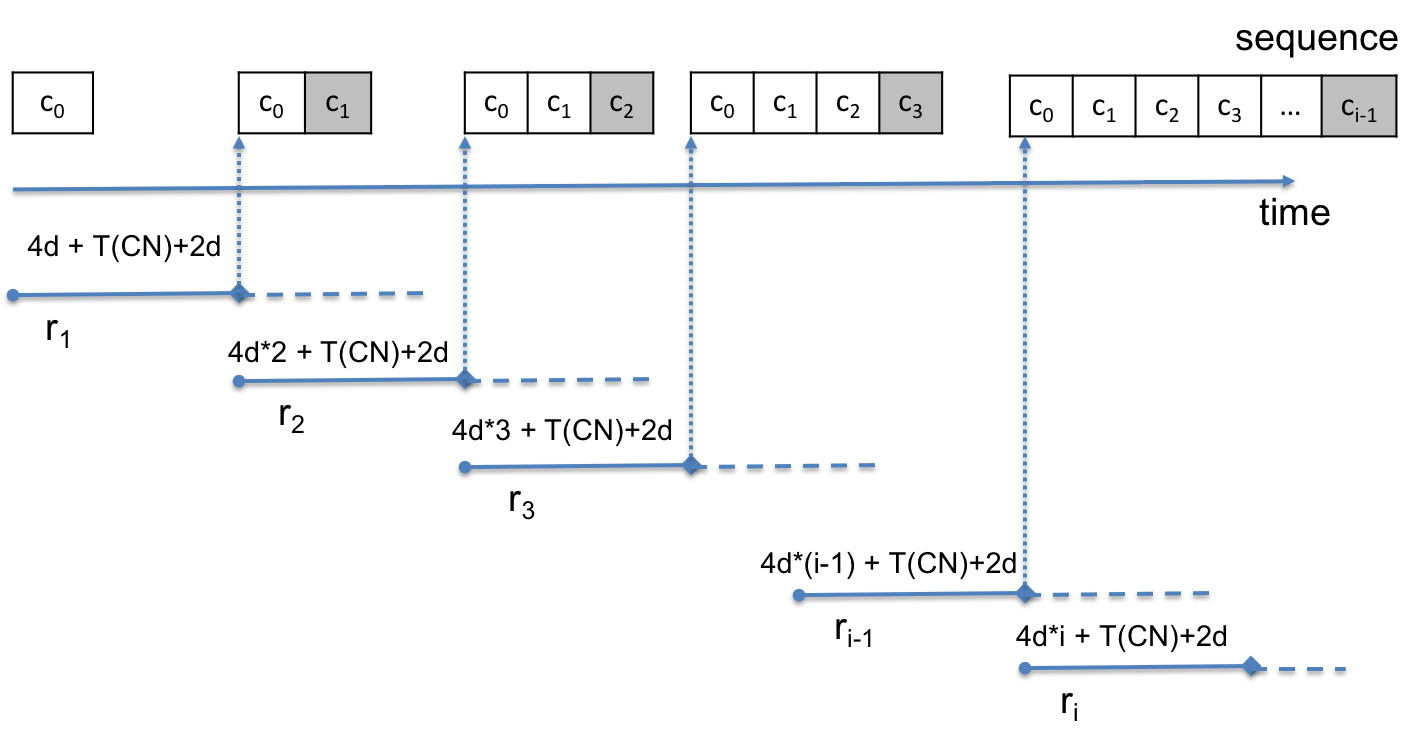
\includegraphics[width=0.60\textwidth]{reconfigExec.png}
		\caption{Successful \act{reconfig} operations.}
		\label{fig:reconfigExec}
	\end{center}
\end{figure}

More formally we can build an execution where all \act{reconfig} operations append their configuration
in the configuration sequence. Consider the partial execution $\EX$ that ends in a state $\state$. Suppose that 
every process $\pr\in\idSet$ knows the same configuration sequence, $\cvec{\pr}{\state}=\cvec{}{\state}$. Also let 
the last finalized operation in $\cvec{}{\state}$ be the last configuration of the sequence, e.g. $\mu(\cvec{}{\state}) = \nu(\cvec{}{\state})$.  
Notice that $\cvec{}{\state}$ can also be the initial configuration sequence $\cvec{\pr}{\state_0}$. 
We extend $\EX_0$ by a series of \act{reconfig} operations, such that each reconfiguration 
$\rec_i$ is invoked by a reconfigurer $r_i$ and attempts to add a configuration $c_i$. 
Let $\rec_1$ be the first reconfiguration that performs the following actions 
without being concurrent with any other \act{reconfig} operation: 
\begin{itemize}
	\item \act{read-config} starting from $\mu(\cvec{}{\state})$
	\item \act{add-config} completing both the consensus proposing $c_1$ and 
	the $\act{put-config}$ action writing the decided configuration
\end{itemize}
%\act{read-config} and \act{add-config} actions without being concurrent 
%with any other operation. 
Since  $\rec_1$ its not concurrent with any other $\act{reconfig}$ operation, then is the only process to propose
a configuration in $\mu(\cvec{}{\state})$,  and hence by the consensus algorithm properties,
$c_1$ is decided. Thus, $\cvec{}{\state}$ is appended by a tuple $\tup{c_1,P}$.

Let now reconfiguration $\rec_2$ be invoked immediately after the completion of the 
$\act{add-config}$ action from $\rec_1$. Since the local sequence at the beginning 
of $\rec_2$ is equal to $\cvec{}{\state}$, then the $\act{read-config}$ action of $\rec_2$
will also start from $\mu(\cvec{}{\state})$.  Since, $\rec_1$ already propagated $c_1$ 
to $\mu(\cvec{}{\state})$ during is $\act{put-config}$ action, then $\rec_2$ will discover 
$c_1$ during the first iteration of its $\act{read-config}$ action, and thus it will 
repeat the iteration on $c_1$. Configuration $c_1$ is the last in the sequence and 
thus the $\act{read-config}$ action of $\rec_2$ will terminate after the second 
iteration.  Following the $\act{read-config}$ action, $\rec_2$ attempts to 
add $c_2$ in the sequence. Since $\rec_1$ is the only reconfiguration that might 
be concurrent with $\rec_2$, and since $\rec_1$ already completed consensus 
in $\mu(\cvec{}{\state})$, then $\rec_2$ is the only operation to run consensus in $c_1$.
Therefore, $c_2$ is accepted and $\rec_2$ propagates $c_2$ in $c_1$ using a 
$\act{put-config}$ action. 

So in general we let configuration $\rec_i$ to be invoked after the completion of 
the $\act{add-config}$ action from $\rec_{i-1}$. As a result, the $\act{read-config}$
action of $\rec_i$ performs $i$ iterations, and the configuration $c_i$ is added 
immediately after configuration $c_{i-1}$ in the sequence. Figure \ref{fig:reconfigExec}
illustrates our execution construction for the reconfiguration operations. 

It is easy to notice that such execution results in the worst case latency for all the 
reconfiguration operations $\rec_1, \rec_2,\ldots, \rec_i$. As by Lemma \ref{lem:rcdelay}
a \act{read-config} action takes at least $4d$ time to complete, then as also 
seen in Figure \ref{fig:reconfigExec}, $k$ reconfigs may take time 
$\opdelay{k} \geq \sum_{i=1}^{k}\left[4\smdelay*i+ \left(\opdelaymin{CN}+2\smdelay\right)\right]$. Therefore, it will take time
$\opdelay{k} \geq 4\smdelay\sum_{i=1}^{k}i+ k\left(\opdelaymin{CN}+2\smdelay\right)$ and the lemma follows.
%
% We can now compute 
% the minimum latency we need to add $k$ new configurations in the configuration 
% sequence starting from the state $\state$ of execution $\EX$.
\end{proof}

The following theorem is the main result of this section, in which we define the relation between $\opdelaymin{CN}$, $d$ and $D$
%show that in any fair execution of ~\ares{}, if the  consensus operations are ``slow enough'' then  
so to guarantee that any read or write issued by a non-faulty client always terminates.

\begin{theorem}
%Consider a  read or  write operation $\pi$, invoked by a non-faulty client, in a fair and well-formed execution of ~\ares{}. Suppose at the point of invocation of $\pi$ the client has $|cseq| = p$. Then if $\opdelaymin{CN} \geq 6D(p + 2) -5d$ the operation $\pi$ completes.
 Suppose  $\opdelaymin{CN} \geq 3(6D-\smdelay)$, then  any  read or write operation $\op$ completes in any execution  $\EX$ of 
\ares{}  for any number of reconfiguration operations in $\EX$.
%$\smdelay \geq \frac{3\lgdelay}{k}-\frac{\opdelay{CN}}{2(k+2)}$
\end{theorem}

\begin{proof}
	By Lemma \ref{lem:configdelay}, 
	$k$ configurations may be installed in:
		$\opdelay{k} \geq 4\smdelay\sum_{i=1}^{k}i+ k\left(\opdelaymin{CN}+2\smdelay\right)$.	
	Also by Lemma \ref{lem:rwdelay}, we know that operation $\op$ takes at most 
$	\opdelay{\op}\leq 6\lgdelay\left(\nu(\cvec{\pr}{\state_e}) - \mu(\cvec{\pr}{\state_s})+2\right)$.
	Assuming that $k=\nu(\cvec{\pr}{\state_e}) - \mu(\cvec{\pr}{\state_s})$, the total number of 
	configurations observed during $\op$, then $\op$ may terminate before a $k+1$ configuration 
	is added in the configuration sequence if 
	  $6\lgdelay(k+2) \leq  4\smdelay\sum_{i=1}^{k}i+ k\left(\opdelaymin{CN}+2\smdelay\right)$ then we have
	  $d \geq \frac{3\lgdelay}{k}-\frac{\opdelaymin{CN}}{2(k+2)}$.
	And that completes the lemma. 
\end{proof}

\remove{

It remains now to examine if a read/write operation may ``catch up'' with any ongoing 
reconfigurations. 
For the sake of a worst case analysis we will assume that reconfiguration operations
may communicate respecting the minimum delay $\smdelay$, whereas read and write 
operations suffer the maximum delay $\lgdelay$ in each message exchange. We will
split our analysis into three directions, with respect to the number of configurations 
installed $k$, and the bound on the minimum delay $\smdelay$:
$(i)$  $k$ is finite, and $\smdelay$ may be unbounded small; $(ii)$ 
$k$ is infinite, and $\smdelay$ may be unbounded small;
$(iii)$  $k$ is infinite, and $\smdelay$ can be bounded.

\myparagraph{$k$ is finite, and $\smdelay$ may be unbounded small.}
In this case we assume a finite number of installed configurations. Also,
as the $\smdelay$ is unbounded, it follows that reconfigurations may be 
installed almost instantaneously. Let us first examine what is the maximum 
delay bound of a any read/write operation. 

\myparagraph{$k$ is infinite, and $\smdelay$ is bounded.}
We will compute the bound on $\smdelay$ with respect to the $\lgdelay$ 
and the number of configurations to be installed $k$ if we want to allow a 
read/write operation to reach ongoing reconfigurations. 

\begin{lemma} \label{lem:delaybound}
	A read/write operation $\op$ may terminate in any execution $\EX$ of 
	\ares{} given that $k$ configurations are installed during $\op$, if
	$
	\smdelay \geq \frac{3\lgdelay}{k}-\frac{\opdelaymin{CN}}{2(k+2)}
	$
\end{lemma}
%\proofremove{
\begin{proof}
	By Lemma \ref{lem:configdelay}, $k$ configurations may be installed in at least:
		$\opdelay{k} \geq 4\smdelay\sum_{i=1}^{k}i+ k\left(\opdelaymin{CN}+2\smdelay\right)$.	
	Also by Lemma \ref{lem:rwdelay}, we know that operation $\op$ takes at most 
$	\opdelay{\op}\leq 6\lgdelay\left(\nu(\cvec{\pr}{\state_e}) - \mu(\cvec{\pr}{\state_s})+2\right)$.
	Assuming that $k=\nu(\cvec{\pr}{\state_e}) - \mu(\cvec{\pr}{\state_s})$, the total number of 
	configurations observed during $\op$, then $\op$ may terminate before a $k+1$ configuration 
	is added in the configuration sequence if 
	  $6\lgdelay(k+2) \leq  4\smdelay\sum_{i=1}^{k}i+ k\left(\opdelaymin{CN}+2\smdelay\right)$ then we have
	  $d \geq \frac{3\lgdelay}{k}-\frac{\opdelaymin{CN}}{2(k+2)}$.
	And that completes the lemma. 
\end{proof}
%}
}

%\begin{theorem*}{\bf \ref{safety:ares:treas}} (Atomicity)
%	Algorithm \ares-\treas{} implements a reconfigurable atomic storage service, given that the 
%	$\act{get-data}$, $\act{get-tag}$, and $\act{put-data}$ primitives used satisfy properties
%	\textbf{C1} and \textbf{C2} of Definition \ref{def:consistency}.
%\end{theorem*}
%
%\begin{proof}
%The figure above \ref{fig:reconfig:ares:treas}
%\end{proof}


\subsection{Storage and Communication Costs for \ares{}.}\label{sec:safety:c}
Storage and Communication costs for \ares{} highly depends on the DAP that we use 
in each configuration. For our analysis we assume that each configuration utilizes the 
algorithms and the DAPs presented in Section \ref{ssec:dap:impl}.
% We now briefly present the storage and communication costs associated with the presented DAPs.
%{\treas{}  %Due to space limitations the proofs appear in \cite{}.

Recall that by our assumption, the storage cost counts the size (in bits) of the coded elements 
%that are locally stored, which are 
stored in variable $List$  at each server. We ignore the storage cost due to meta-data.
For  communication cost we measure the bits sent on the wire between the nodes.

\begin{lemma}\label {thm:storage_TREAS}
	The worst-case total storage cost of Algorithm \ref{fig:casopt} is $(\delta +1 )\frac{n}{k}$.
\end{lemma}
\begin{proof}
  The maximum number of  (tag, coded-element) pair in the $List$ is $\delta+1$, and the size of each coded element is 
  $\frac{1}{k}$ while the tag variable is a metadata and therefore, not counted. So, the total storage cost is $(\delta +1)\frac{n}{k}$.
\end{proof}

We next state  the communication cost for the write and read operations in  Aglorithm \ref{fig:casopt}. Once again, note that we ignore the communication cost arising from exchange of meta-data.

\begin{lemma} \label{treas:write_cost}
	The communication cost associated with a successful  write operation in Algorithm \ref{fig:casopt} is at most $\frac{n}{k}$. 
\end{lemma}

\begin{proof}
  During read operation, in the $\act{get-tag}$ phase the servers respond with their highest tags variables, which are metadata. However, in the $\act{put-data}$ phase, the reader sends each server the  coded elements of size  $\frac{1}{k}$ each, and hence the total cost of communication for this is $\frac{n}{k}$. Therefore, we have the worst case communication cost of a write operation is $ \frac{n}{k}$.
\end{proof}

\begin{lemma} \label{radonc:read_cost}
	The communication cost associated with a successful read operation in Algorithm \ref{fig:casopt} is at most $(\delta +2)\frac{n}{k}$. 
\end{lemma}
\begin{proof}
  During read operation, in the $\act{get-data}$ phase the servers respond with their $List$ variables and hence each such list 
  is of size at most $(\delta +1)\frac{1}{k}$, and then counting all such responses give us $(\delta +1)\frac{n}{k}$.  In the $\act{put-data}$ phase, the reader sends each server the  coded elements of size  $\frac{1}{k}$ each, and hence the total cost of communication for this is $\frac{n}{k}$. Therefore, we have the worst case communication cost of a read operation is 
  $(\delta+2) \frac{n}{k}$.
\end{proof}

From the above Lemmas we get.

\begin{theorem}\label{treas:performance}
 The \ares{} algorithm has: (i) storage cost $(\delta +1 )\frac{n}{k}$, (ii) communication 
cost for each write at most to $\frac{n}{k}$, and (iii) communication 
cost for each read at most $(\delta +2)\frac{n}{k}$.
\end{theorem}
